%--------------------------------------------
% Univerzitet u Tuzli
% Fakultet elektrotehnike
% Tehnologije za podršku tehničkom pisanju
% Selimbašić Kemal
% Br. indeksa - 20191
% Zadaća 1
%--------------------------------------------


\documentclass[a4paper,10pt]{article}
\usepackage[utf8]{inputenc}
\usepackage[left=24mm, right=30mm, top=25mm, bottom=25mm]{geometry}
\usepackage[T1]{fontenc}
\usepackage[english]{babel}
\usepackage{color}
\usepackage[shadow,textwidth=20mm,color=color1,bordercolor=black,linecolor=color1]{todonotes}
\usepackage{soul}
\usepackage{fancyhdr}
\usepackage{graphicx}
\usepackage{amsmath}
\usepackage{mathtools}
\usepackage{fix-cm}
\usepackage[pdftex]{hyperref}
\usepackage{multirow}
\usepackage{colortbl}
\usepackage{array}
\usepackage{enumerate}
\usepackage{caption}
\usepackage{listings}
\usepackage{setspace}
\usepackage{tikz}
\usepackage{xcolor}
\usepackage[american]{circuitikz}
\usetikzlibrary{arrows,shapes,positioning}
\usetikzlibrary{circuits.logic.US}
\usetikzlibrary{calc} 
\usetikzlibrary{patterns} 
\usepackage{pgfplots}
\pgfplotsset{compat=1.14}
\usepackage{pgfkeys}
\usepackage{embedfile}



\embedfile{logo.pdf}


\newcommand{\bluetext}[1]
{\texttt{\color{blue}#1}\color{black}~}


\fancypagestyle{fet_style}
{	\lhead{\small{\textsc{Selimbašić Kemal}}} \chead{}	\rhead{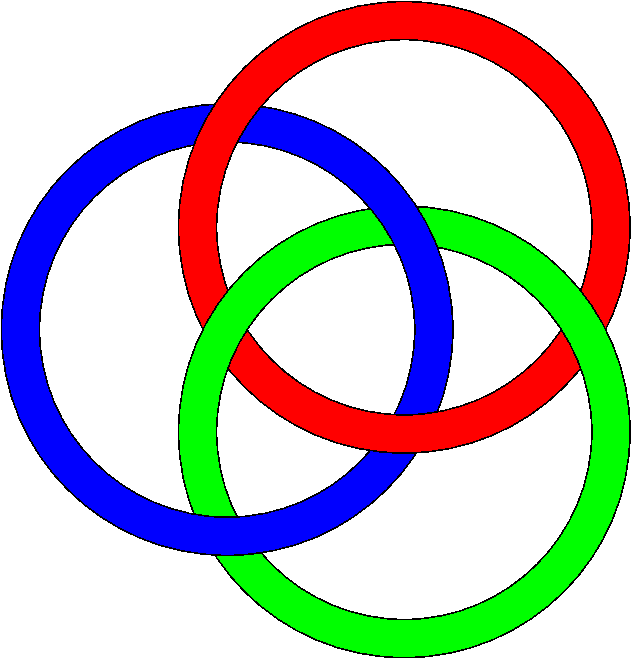
\includegraphics[scale=0.06,trim={0.25mm 0.25mm 0.25mm 0.25mm},clip=true]{logo.pdf}}
	\lfoot{} \cfoot{\thepage} \rfoot{}
  	\renewcommand{\headrulewidth}{0.25pt}
  	\renewcommand{\footrulewidth}{0pt}}
\pagestyle{fet_style}



\definecolor{color1}{RGB}{230,230,250}
\definecolor{color2}{RGB}{216,123,109}
\definecolor{color3}{RGB}{245,245,144}
\definecolor{color4}{RGB}{195,42,20}
\definecolor{color5}{RGB}{32,185,240}
\definecolor{color6}{RGB}{237,7,142}




\begin{document}
\noindent{}\rmfamily{Univerzitet u Tuzli} \hfill{}	\textsc{Proljeće 2021.} \\
\rmfamily{Fakultet elektrotehnike \hfill{}	Selimbašić Kemal \\ TK001}



\vspace{5mm}
\begin{center}
    \LARGE{}\textsc{Tehnologije za Podršku Tehničkom Pisanju Zadaća I}	\todo[]{\scriptsize{Naslov doku-ment ver-tikalno je pomjeren za 5 mm u odnosu na prethodni i naredni sadržaj.}}
    \vspace{5mm}



    \renewcommand{\abstractname}{Abstract}
    \begin{abstract}
        \textbf{\textsl{U okviru zadaće}} pokušat ćete demonstrirati svo stečeno znanje iz predmeta \textsl{Tehnologije za podršku tehničkom pisanju} vezano za \LaTeX. Bez VARANJA, replicirati sadržaj dokumenta (stranice od 1 do 6) pri čemu se mora obratiti pažnja na svaki detalj u originalnom dokumentu. Replicirani dokument mora biti \underline{vjerodostojna kopija} originalnom dokument u (100\% kopija osim dijela prezime i ime, i broj indeksa). Kako rezultat, studenti će \textbf{\textsl{\color{blue}predati kod}} (\textsl{*.tex i *.pdf file}).
    \end{abstract}
\end{center}



\renewcommand{\contentsname}{Kratak sadržaj}
\renewcommand{\listfigurename}{Lista slika}
\renewcommand{\listtablename}{Lista tabela}
\renewcommand{\figurename}{Sličica}
\renewcommand{\tablename}{Tabelica}
\tableofcontents
\listoffigures
\listoftables



\section{Stil dokumenta}
Redeniranjem funkcionalnosti komande {\color{color2}{\verb|\contentsname{}|}} promijeniti naziv liste sadržaja u \textsl{Kratak sadržaj.}  Na sličan način ponoviti za komande {\color{color2}{\verb|\listfigurename{}|}}, {\color{color2}{\verb|\listtablename{}|}}, {\color{color2}{\verb|\figurename{}|}} i {\color{color2}{\verb|\tablename{}|}} uslijed nedostatka podrške za govorno područje Bosne i Hercegovine u paketu babel.



\newpage
\pagestyle{fet_style}
\subsection{Margine dokumenta}
Margine stranica dokumenta su postavljene na sljedeći način: lijeva 24 mm, donja na 25 mm i gornja na 25 mm a desna na 30 mm. Na mjesto \textsl{Prezime Ime} upisat vaše \underline{ime i prezime.} {\color{color2}\textsl{Obratiti pažnju}} da se na tekućoj i narednim stranicama dokumenta zadaće, nalazi zaglavlje i podnožje a na prethodnoj ne! U okviru zadaće kreirati \LaTeX  komande i okruženja samo na mjestima gdje to ima smisla.



\subsection{Zaglavlje i podnožje dokumenta}
\textrm{Stil dokumenta generirati sa komandama iz paketa \texttt{fancyhdr} pri čemu će se novi stil zvati \texttt{fet\_style}. Slika unutar zaglavlja stranice dokumenta (\textsl{logo.pdf}), skalirana je na 0.06 a prostor oko slike skraćen je za 0.25 mm sa svih strana} \todo[]{\scriptsize{Upotrijebiti \texttt{trim} \& \texttt{clip} opcije}} . Debljina linije u zaglavlju je 0.25 pt.



\section{Matematički mod i tabele}
\subsection{Matematički mod}
Tokom semestra, u \LaTeX-u smo upoznali matematički mod\footnote{{\color{color2}{\textsl{Ne zaboravite}}} da matematički mod zahtjeva uključenje paketa \texttt{amsmath}.} koji nam omogućava i formatiranje matrica\footnote{Adjungovana matrica je odmaknuta za 3mm od gornjeg i donjeg paragrafa.} \\ \hfill{}
\vspace{3mm}
\begin{center}
    \normalsize
    $
        \textbf{adj}
        \begin{pmatrix}
            \alpha_{11} & \alpha_{12} & \alpha_{13} \\[6pt]
            \alpha_{21} & \alpha_{22} & \alpha_{23} \\[6pt]
            \alpha_{31} & \alpha_{32} & \alpha_{33}
        \end{pmatrix} =
        \begin{pmatrix} +
            \begin{vmatrix}
                \alpha_{22} & \alpha_{23} \\[6pt]
                \alpha_{32} & \alpha_{33}
            \end{vmatrix}  & -
            \begin{vmatrix}
                \alpha_{12} & \alpha_{13} \\[6pt]
                \alpha_{32} & \alpha_{33}
            \end{vmatrix}  & +
            \begin{vmatrix}
                \alpha_{12} & \alpha_{13} \\[6pt]
                \alpha_{22} & \alpha_{23}
            \end{vmatrix}      \\ \\-
            \begin{vmatrix}
                \alpha_{21} & \alpha_{23} \\[6pt]
                \alpha_{31} & \alpha_{33}
            \end{vmatrix}  & +
            \begin{vmatrix}
                \alpha_{11} & \alpha_{13} \\[6pt]
                \alpha_{31} & \alpha_{33}
            \end{vmatrix}  & -
            \begin{vmatrix}
                \alpha_{11} & \alpha_{13} \\[6pt]
                \alpha_{21} & \alpha_{23}
            \end{vmatrix}      \\[6pt] \\+
            \begin{vmatrix}
                \alpha_{21} & \alpha_{22} \\[6pt]
                \alpha_{31} & \alpha_{32}
            \end{vmatrix}  & -
            \begin{vmatrix}
                \alpha_{11} & \alpha_{12} \\[6pt]
                \alpha_{31} & \alpha_{32}
            \end{vmatrix} & +
            \begin{vmatrix}
                \alpha_{11} & \alpha_{12} \\[6pt]
                \alpha_{21} & \alpha_{22}
            \end{vmatrix}
        \end{pmatrix} $
\end{center}
\vspace{3mm}


\noindent{}U nastavku imamo primjer proračuna \texttt{LLR} duo-binarnog turbo-konvolucionog dekodera za slučaj \texttt{MAP} algoritma:
\begin{equation}
    L\left(u_{k}\right)=\ln \left(\frac{\sum_{n, m=u_{k}} \tilde{\alpha}_{k}^{n, m} \cdot \tilde{\beta}_{k+1}^{n, m} \cdot \exp \left(\frac{L_{c}}{2}\left(y_{k}^{s, 1} c_{k}^{s, 1}+y_{k}^{s, 2} c_{k}^{s, 2}+y_{k}^{p, j} c_{k}^{p, j}\right)\right) \cdot e^{L_{a}^{m}\left(u_{k}\right)}}{\sum_{n, m=00} \tilde{\alpha}_{k}^{n, m} \cdot \tilde{\beta}_{k+1}^{n, m} \cdot \exp \left(\frac{L_{c}}{2}\left(y_{k}^{s, 1} c_{k}^{s, 1}+y_{k}^{s, 2} c_{k}^{s, 2}+y_{k}^{p, j} c_{k}^{p, j}\right)\right)}\right)
\end{equation}



\noindent{}U sljedećem redu ispisan je datum zadaće Rimskim brojevima koristeći familiju fonta \textsl{New Century Schoolbook (pnc)} visine \textsl{75 pt}\footnote{Obratiti pažnju da će nam trebati paket \texttt{fix-cm}\vspace{28mm}}
\vspace{10mm}
\begin{center}
    \fontsize{75pt}{6.5mm}\fontfamily{pnc}\selectfont{MMXXI.IV.II.}
\end{center}



\newpage
\subsection{Tabele}
U nastavku imamo tri table postavljene koristeći okruženje \bluetext{minipage}, \bluetext{tabular}i \bluetext{table}. Za tabele je redenirana funkcionalnost komande {\color{color2}{\verb|\arraystretch{}|}} na vrijednost 1.1
\begin{table}[h]
    \centering{}\small{}
    \setstretch{1.1}
    \begin{tabular}{c c c c c}
        \hline \hline
        \rowcolor[RGB]{77,77,77}\multicolumn{2}{c}{\color{white}Materijal} & \color {white}\textsl{W(0)[eV]} & \color{white}$\alpha[e V / K]$ & \color{white}$\beta[\boldsymbol{K}$]       \\ \hline \hline
        \rowcolor[RGB]{242,242,242} Si                                     & Sicilij                         & 1.17                           & $4.73 \cdot 10^{-4}$                 & 636 \\
        Ge                                                                 & Germanijum                      & 0.74                           & $4.77 \cdot 10^{-4}$                 & 235 \\
        \rowcolor[RGB]{242,242,242} GaAs                                   & Galijum Arsenid                 & 1.52                           & $5.41 \cdot 10^{-4}$                 & 204 \\
        AlAs                                                               & Aluminijum Sulfid               & 2.24                           & $6.00 \cdot 10^{-4}$                 & 408 \\
        \rowcolor[RGB]{242,242,242} InAs                                   & Indijum Arsenid                 & 0.42                           & $2.50 \cdot 10^{-4}$                 & 75  \\
        InP                                                                & Indijum Fostat                  & 1.42                           & $3.36 \cdot 10^{-4}$                 & 162 \\
        \rowcolor[RGB]{242,242,242} GaP                                    & Galijum Fosfat                  & 2.33                           & $5.77 \cdot 10^{-4}$                 & 372 \\\hline \hline
    \end{tabular}
    \caption{Širina zabranjene zone ${\Delta}W(T)$ poluprovodnika je temperaturno zavisna}
    \label{Tabelica:tab1}
\end{table}\\[1mm] \hfill{}



\begin{minipage}[t]{0.45\textwidth}
    \centering{}
    \setstretch{1.1}
    \begin{tabular}{c c c}
        \hline \hline
        \rowcolor[RGB]{77,77,77}\color {white}BAZA & \color{white}BROJNI SISTEM & \color {white}CIFRE         \\ \hline \hline
        2                                          & Binarni                    & 0,1                         \\
        \rowcolor[RGB]{242,242,242} 3              & Ternarni                   & 0,1,2                       \\
        5                                          & Kvinarni                   & $0,1,\hdots,4$              \\
        \rowcolor[RGB]{242,242,242} 8              & Oktalni                    & $0,1,\hdots,7$              \\
        10                                         & Dekadski                   & $0,1,\hdots,9$              \\
        \rowcolor[RGB]{242,242,242} 12             & Duodekani                  & $0,1,\hdots,9,\alpha,\beta$ \\
        16                                         & Heksadekadski              & $0,1,\hdots,9$,A,$\hdots$,F \\ \hline \hline
    \end{tabular}
    \captionof{table}{Pozicioni brojni sistemi}
    \label{Tabelica:tab2}
\end{minipage}
\begin{minipage}[t]{0.45\textwidth}
    \centering{}
    \setstretch{1.1}
    \begin{tabular}{|l|c|r|}
        \hline \hline
        \cellcolor[RGB]{204,255,204}L1                        & L2                            & L3 \\ \hline
        \multirow{2}{*}{MR2}                                  & \multicolumn{2}{c|}{MC2}           \\ \cline{2-2} & D & \cellcolor[RGB]{255,230,204}E \\ \hline
        G                                                     & \cellcolor[RGB]{255,204,204}E & M  \\ \hline
        \multicolumn{2}{|c|}{\cellcolor[RGB]{204,204,255}MC1} & \multirow{2}{*}{MR1}               \\ \cline{1-2} A & B & \\ \hline \hline
    \end{tabular}
    \captionof{table}{Spajanje ćelija}
    \label{Tabelica:tab3}
\end{minipage}\hfill{}



\begin{center}
    \fbox{\colorbox{color3}{\parbox{151mm}{U malom ograničenom paragrafu širine 151 mm prikazana je lista malih Grčkih karaktera, velikih rimskih cifara\footnote{} i heksadecimalnih cifara\footnote{}
                \begin{enumerate}[a)]
                    \item \small{}$\alpha, ~\Delta, ~\sigma, ~\Gamma, ~\rho, ~\Psi, ~\mu, ~\gamma, ~\epsilon, ~\Omega, ~\psi, ~\pi, ~\kappa, ~\vartheta, ~\delta, ~\omega, ~\lambda, ~\tau.$
                    \item $I$, $V$, $X$, $L$, $D$, $C$ i $M$
                    \item \scriptsize{\texttt{0, 1, 2, 3, 4, 5, 6, 7, 8, 9, A, B, C, D, E i F}}
                \end{enumerate}}}}
\end{center}



Sistem linearnih diferencijalnih jednačina koji opisuju ponašanje jednog električnog sistema je:
$$
    \begin{array}{l}
        y_{1}^{\prime}(x)=b_{1}(x)+a_{1,1}(x) y_{1}+\cdots+a_{1, n}(x) y_{n} \\
        \vdots                                                               \\
        y_{n}^{\prime}(x)=b_{n}(x)+a_{n, 1}(x) y_{1}+\cdots+a_{n, n}(x) y_{n}
    \end{array}
$$



\section{Paketi za crtanje u \LaTeX-u}
\subsection{TikZ paket}
Na slici 1 je prikazan talansi oblik diferencijalnog 2irinski modularnog (PWM) signala na ulazu Xilix FPGA chipa XC6SLX9-TQG144. Za crtanje konkretnih krivi koristiti komandu {\color{color2}{\verb|\addplot{}|}}.
\newpage
\begin{figure}
    \centering
    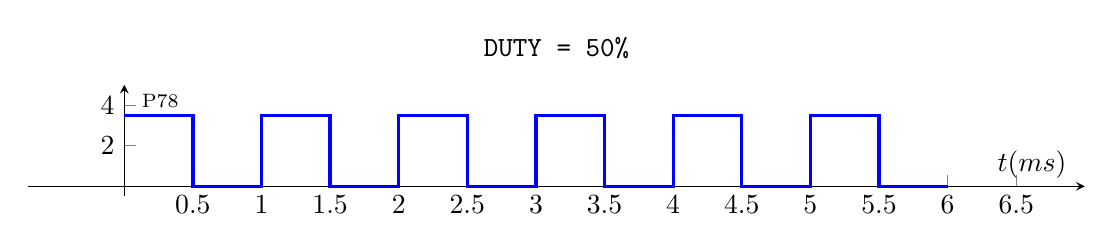
\begin{tikzpicture}
        \begin{axis}[
                width=15cm,
                height=3cm,
                x axis line style={-stealth},
                y axis line style={-stealth},
                x label style={at={(axis description cs:0.95,0.5)},anchor=north},
                y label style={at={(axis description cs:0.125,1)},rotate=-90,anchor=north},
                title={\texttt{DUTY = 50\%}},
                xticklabels={0.5, 1, 1.5, 2, 2.5, 3, 3.5, 4, 4.5, 5, 5.5, 6, 6.5},
                xlabel={$t(ms)$},
                ylabel={\scriptsize{P78}},
                ymax=5,xmax=7,
                axis lines*=center,
                ytick={2,4},
                xtick={0.5, 1, 1.5, 2, 2.5, 3, 3.5, 4, 4.5, 5, 5.5, 6, 6.5}]
            \addplot+[very thick,mark=none,const plot]
            coordinates
                {(0,3.5) (0.5,0) (1,3.5) (1.5,0) (2,3.5) (2.5,0) (3,3.5) (3.5,0) (4,3.5) (4.5,0) (5,3.5) (5.5,0) (6,0)};
        \end{axis}
    \end{tikzpicture}
    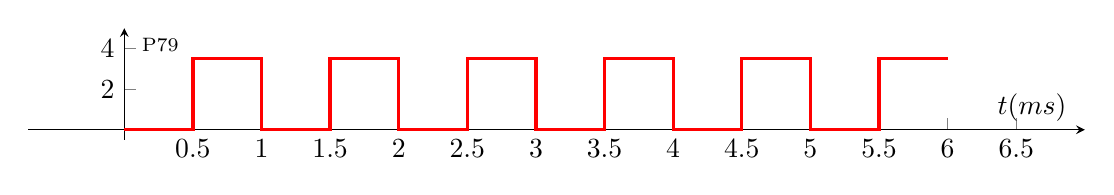
\begin{tikzpicture}
        \begin{axis}[
                width=15cm,
                height=3cm,
                x axis line style={-stealth},
                y axis line style={-stealth},
                x label style={at={(axis description cs:0.95,0.5)},anchor=north},
                y label style={at={(axis description cs:0.125,1)},rotate=-90,anchor=north},
                xticklabels={0.5, 1, 1.5, 2, 2.5, 3, 3.5, 4, 4.5, 5, 5.5, 6, 6.5},
                xlabel={$t(ms)$},
                ylabel={\scriptsize{P79}},
                ymax=5,xmax=7,
                axis lines*=center,
                ytick={2,4},
                xtick={0.5, 1, 1.5, 2, 2.5, 3, 3.5, 4, 4.5, 5, 5.5, 6, 6.5}]
            \addplot+[very thick,mark=none,const plot, color=red]
            coordinates
                {(0,0) (0.5,3.5) (1,0) (1.5,3.5) (2,0) (2.5,3.5) (3,0) (3.5,3.5) (4,0) (4.5,3.5) (5,0) (5.5,3.5) (6,3.5)};
        \end{axis}
    \end{tikzpicture}
    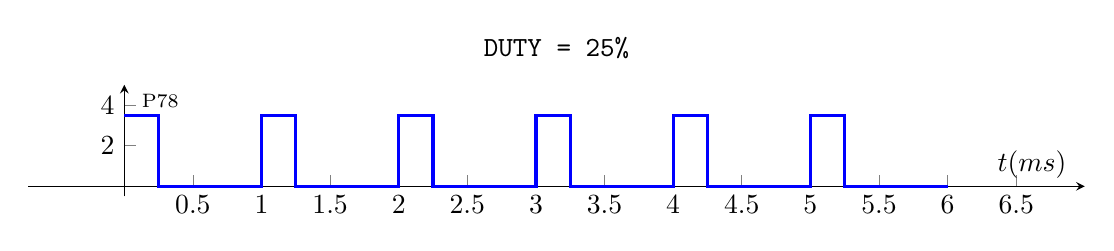
\begin{tikzpicture}
        \begin{axis}[
                width=15cm,
                height=3cm,
                x axis line style={-stealth},
                y axis line style={-stealth},
                x label style={at={(axis description cs:0.95,0.5)},anchor=north},
                y label style={at={(axis description cs:0.125,1)},rotate=-90,anchor=north},
                title={\texttt{DUTY = 25\%}},
                xticklabels={0.5, 1, 1.5, 2, 2.5, 3, 3.5, 4, 4.5, 5, 5.5, 6, 6.5},
                xlabel={$t(ms)$},
                ylabel={\scriptsize{P78}},
                ymax=5,xmax=7,
                axis lines*=center,
                ytick={2,4},
                xtick={0.5, 1, 1.5, 2, 2.5, 3, 3.5, 4, 4.5, 5, 5.5, 6, 6.5}]
            \addplot+[very thick,mark=none,const plot]
            coordinates
                {(0,3.5) (0.25,0) (1,3.5) (1.25,0) (2,3.5) (2.25,0) (3,3.5) (3.25,0) (4,3.5) (4.25,0) (5,3.5) (5.25,0) (6,0)};
        \end{axis}
    \end{tikzpicture}
    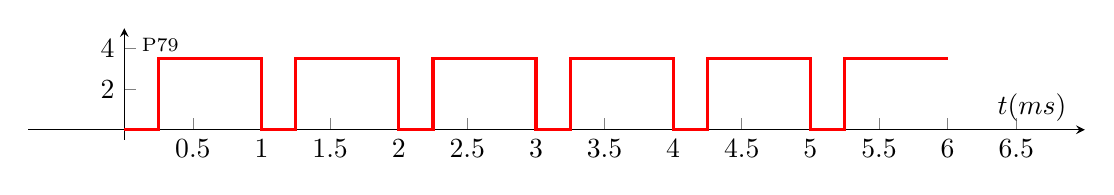
\begin{tikzpicture}
        \begin{axis}[
                width=15cm,
                height=3cm,
                x axis line style={-stealth},
                y axis line style={-stealth},
                x label style={at={(axis description cs:0.95,0.5)},anchor=north},
                y label style={at={(axis description cs:0.125,1)},rotate=-90,anchor=north},
                xticklabels={0.5, 1, 1.5, 2, 2.5, 3, 3.5, 4, 4.5, 5, 5.5, 6, 6.5},
                xlabel={$t(ms)$},
                ylabel={\scriptsize{P79}},
                ymax=5,xmax=7,
                axis lines*=center,
                ytick={2,4},
                xtick={0.5, 1, 1.5, 2, 2.5, 3, 3.5, 4, 4.5, 5, 5.5, 6, 6.5}]
            \addplot+[very thick,mark=none,const plot, color=red]
            coordinates
                {(0,0) (0.25,3.5) (1,0) (1.25,3.5) (2,0) (2.25,3.5) (3,0) (3.25,3.5) (4,0) (4.25,3.5) (5,0) (5.25,3.5) (6,3.5)};
        \end{axis}
    \end{tikzpicture}
    \caption{Talasni oblik diferencijanog PWM signala na ulazu jednog digitalnog sistema}
    \label{Slicica:fig1}
\end{figure}




\begin{figure}
    \begin{minipage}{0.5\textwidth}\centering{}
        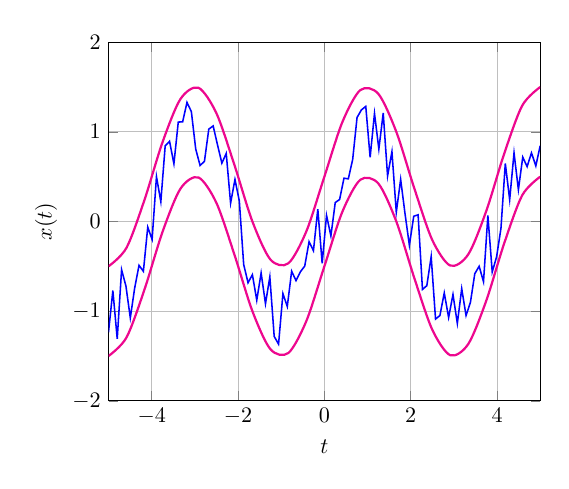
\begin{tikzpicture}[scale=0.8]
            \begin{axis}[xlabel=$t$,ylabel=$x(t)$,xmin=-5,xmax=5,ymin=-2,ymax=2,grid=major,grid style={solid}]
                \addplot[color6,line width=1pt,smooth] expression{(sin(90*x))+0.5};
                \addplot[domain=-5:5,blue,samples=100,line width=0.7pt] expression{sin(90*x)+0.4*rand};
                \addplot[color6,line width=1pt, smooth]expression{(sin(90*x))-0.5};
            \end{axis}
        \end{tikzpicture}
        \caption{Sinusne funkcije sa i bez izobličenja}
        \label{Slicica:fig2}
    \end{minipage}
    \begin{minipage}{0.5\textwidth}\centering{}
        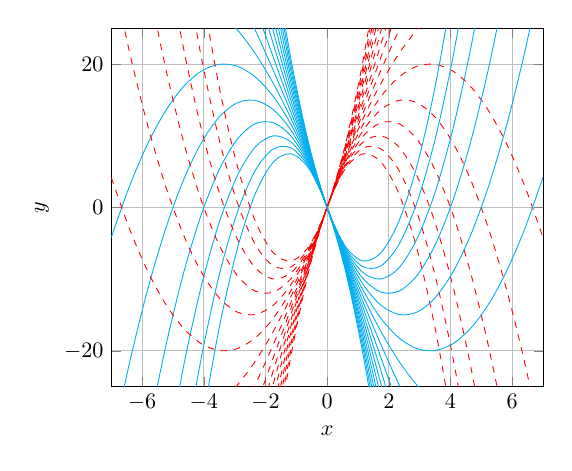
\begin{tikzpicture}[scale=0.8]
            \pgfplotscreateplotcyclelist{pft}{
                red,dashed\\
                cyan,solid\\
            }
            \begin{axis}[xlabel=$x$,ylabel=$y$,xtick={-6,-4,...,6},ytick={-20,0,20},xmin=-7,xmax=7,ymin=-25,ymax=25,grid=major,grid style={solid},cycle list name=pft]
                \pgfplotsinvokeforeach{-2.4,-2.1,...,2.4}{
                    \addplot+[no marks,domain=-7:7,smooth]{2*#1*x*x+12*x};
                    \addplot+[no marks,domain=-7:7,smooth]{2*#1*x*x-12*x};};
            \end{axis}
        \end{tikzpicture}
        \caption{Serija parabola}
        \label{Slicica:fig3}
    \end{minipage}
\end{figure}\vspace{1mm}\hfill

\noindent{}Sinusni signali oblika $x(t)=\sin (90 t)+0.4 \cdot \text { rand } i y(t)=\sin (90 t) \pm 0.5$ kreirane su sa okruženjem \bluetext{tikzpicture} i \bluetext{axis} i prikazani na slici 3.1. Za crtanje konkretnih krivi koristiti komandu {\color{color2}{\verb|\addplot{}|}}. Aktiviranje mrežice na grafiku izvodimo sa opcijom \texttt{grid}. Postavke opsega grafika (\textsl{plot-a}) su \texttt{xmin=-5, xmax=5, ymin=-2 i ymax=2} u okviru \bluetext{axis} okruženja. \\
Na slici \ref{Slicica:fig3} prikazana je serija parabola oblika $y=2 a x^{2} \pm 12 x$ kreiranih sa okruženjem \bluetext{tikzpicture}  i \bluetext{axis}. Serija parabola nacrtana je za opseg vrijednosti $a=\{-2.4,-2.1, \ldots, 2.4\}$. Za crtanje serije parabola koristiti komandu {\color{color2}{\verb|\addplot{}|}} u sklopu komande {\color{color2}{\verb|\foreach{}|}} koja ima varijablu \texttt{a} koja  se mijenja u skladu sa prethodno definiranim opsegom i korakom. Obratiti pažnju da su neke krive markirane sa crvenom bojom (isprekidana linija) a neke plavom\footnote{Obratiti pažnju na boje kao i njihove nijanse, u dokumentu.}.



\subsection{Električne, blok sheme i {\color{color4}\textsl{circuitikz}} paket}
Na slici \ref{Slicica:fig4} prikazana je implementacija 2/4 digitalnog multipleksera sa osnovnim logičkim kolima\footnote{Prilikom crtanja logičke sheme neophodno je uključiti \textsl{tikz} biblioteku \textsl{circuits.logic.US} }. Ukoliko imate poteškoća sa realizacijom logičke i električne sheme, možete se poslužiti primjerima iz kratkog \textsl{manuala} \texttt{circutikz} paketa, koje se nalazi na \texttt{CTAN} {\color{color5}\href{https://texdoc.org/missing.html}{stranici}}.



\newpage
\begin{figure}[h]
    \centering{}
    \begin{circuitikz}[circuit logic US,scale=0.8]
        small{
                \draw (0,0)node[above]{A}--(0,-8);
                \draw (1.5,0)node[above]{B}--(1.5,-8);
                \draw (2.5,0)node[above]{E}--(2.5,-8);}
        \draw (-0.7,-1.5)node[not gate,logic gate inputs=n,scale=1,very thick,rotate=-90](ne1){};
        \draw (0.7,-1.5)node[not gate,logic gate inputs=n,scale=1,very thick,rotate=-90](ne2){};
        \draw (4,-3)node[and gate,logic gate inputs=nnn,scale=1,very thick](i1){};
        \draw (4,-4.5)node[and gate,logic gate inputs=nnn,scale=1,very thick](i2){};
        \draw (4,-6)node[and gate,logic gate inputs=nnn,scale=1,very thick](i3){};
        \draw (4,-7.5)node[and gate,logic gate inputs=nnn,scale=1,very thick](i4){};
        \draw (0,-0.5)--(-0.7,-0.5)to[short,-](ne1.input);
        \draw (1.5,-0.5)--(0.7,-0.5)to[short,-](ne2.input);
        \draw [short,-](ne1.output)--(-0.7, -8);
        \draw [short,-](ne2.output)--(0.7, -8);
        \draw (-0.7,-2.8)to[short,*-](i1.input 1);
        \draw (0.7,-3)to[short,*-](i1.input 2);
        \draw (2.5,-3.2)to[short,*-](i1.input 3);
        \draw (i1.output)--(6,-3)node[right]{$D_0$};
        \draw (-0.7,-4.3)to[short,*-](i2.input 1);
        \draw (1.5,-4.5)to[short,*-](i2.input 2);
        \draw (2.5,-4.7)to[short,*-](i2.input 3);
        \draw (i2.output)--(6,-4.5)node[right]{$D_1$};
        \draw (0,-5.8)to[short,*-](i3.input 1);
        \draw (0.7,-6)to[short,*-](i3.input 2);
        \draw (2.5,-6.2)to[short,*-](i3.input 3);
        \draw (i3.output)--(6,-6)node[right]{$D_2$};
        \draw (0,-7.3)to[short,*-](i4.input 1);
        \draw (1.5,-7.5)to[short,*-](i4.input 2);
        \draw (2.5,-7.7)to[short,*-](i4.input 3);
        \draw (i4.output)--(6,-7.5)node[right]{$D_3$};
    \end{circuitikz}
    \caption{Implementacija 2/4 digitalnog multipleksera sa osnovnim logičkim kolima.}
    \label{Slicica:fig4}
\end{figure}\hfill{}



\noindent{}Na slici \ref{Slicica:fig4} je prikazana shema električnog kola koje ispoljava osobine klasične teorije haosa\footnote{Za više detalja pogledati {\color{color5}\href{https://www-inst.cs.berkeley.edu/~ee129/sp10/handouts/GenesisChuasCircuit.pdf}{stranici}}}.U osnovi
\textsl{Chua elektronički sklop }predstavlja \textsl{aperiodični oscilator} koji proizvodi naizmjenični signal čije se vrijednosti nikada ne ponavljaju. Za kreiranje električne sheme na slici \ref{Slicica:fig4} koristiti okruženje \bluetext{circuitikz} i komponente \texttt{R, L, C, D, ground i op amp}. Za pravilno kreiranje spojnica kod {\color{color2}{\verb|\draw{}|}} komande možete koristiti komandu {\color{color2}{\verb|\let{}|}}\footnote{Pogledati primjer na predavanju tptp\textunderscore8.pdf na stranici 15}.



\begin{figure}[h]
    \centering{}
    \begin{circuitikz}[circuit logic US,american,cute inductors,scale=1.5]
        \normalsize{}
        \draw (-0.5,0) to[R, l=$R_1$,*-*](1.5,0);
        \draw (-0.5,0)--(-2,0)to[short](-2,-0.7);
        \draw (-0.5,0) to[C, l_=$C_1$,-*] (-0.5,-3);
        \draw (2,-3)--(-2,-3)to[short](-2,-2.2);
        \draw (1.5,0) to[C,l_=$C_2$,-*] (1.5,-3);
        \draw (-2,-0.7) to[L, l_=$L_1$] (-2,-2.2);
        \draw (3,-2) to[R, l_=$R_2$](3,-2.7);
        \draw (3,-0.8) to[D*, l=$D_1$](3,-0.4);
        \draw (1.5,0)to[short,-*](3,0);
        \draw (1.5,-3)to[short,-*](3,-3);
        \draw (3,0)to[short](3,-0.4);
        \draw (3,-3)to[short](3,-2.7);
        \draw (3,-2)to[short](3,-0.8);
        \draw (4.5,-2) to[R, l=$R_3$](4.5,-2.7);
        \draw (4.5,-0.4) to[D*, l=$D_2$](4.5,-0.8);
        \draw (4.5,-3)to[short](4.5,-2.7);
        \draw (4.5,-2)to[short](4.5,-0.8);
        \draw (3,0)to[short,-*](4.5,0);
        \draw (3,-3)to[short,-*](4.5,-3);
        \draw (4.5,-0.4)to[short,-*](4.5,0);
        \draw (4.5,-3)node[ground](){};
        \draw (5.5,-0.4)to[R, l_=$R_4$](6.5,-0.4);
        \draw (5.5,-2.5)to[R, l=$R_5$](6.5,-2.5);
        \draw (5.8,-3)to[R, l_=$R_6$](6.8,-3);
        \draw (7.6,-1.5) node[op amp,rotate=180] (opamp) {};
        \draw (8.4,-0.4)to[short](opamp.+);
        \draw (8.4,-2.5)to[short](opamp.-);
        \draw (6.5,-0.4)to[short,-*](8.4,-0.4);
        \draw (6.5,-2.5)to[short,-*](8.4,-2.5);
        \draw (5.5,-1.5)to[short,*-](opamp.out);
        \draw (5.5,-1.5)to[short](5.5,-0.4);
        \draw (5.5,-1.5)to[short](5.5,-2.5);
        \draw (5.8,-3)to[short](4.5,-3);
        \draw (6.8,-3)to[short](8.4,-3)--(8.4,-2.5);
        \draw (4.5,0)to[short](8.4,0)--(8.4,-0.4);
    \end{circuitikz}
    \caption{Električna shema Chua elektroničkog sklopa}
    \label{Slicica:fig5}
\end{figure}
\noindent{}Slika \ref{Slicica:fig5} predstavlja model jednog komunikacijskog sistema. Prilikom crtanja modela i ostalih tikz baziranih dijagrama/grafika/slika možete se poslužiti aplikacijama kao što je \textsl{ktikz, QTikZ, TpX} i sl.



\newpage
\begin{figure}[h]\centering
    \pgfdeclareradialshading{spherebrown}{\pgfpoint{-0.8cm}{1cm}}
    {rgb(0cm)=(1,1,1);
        rgb(1.5cm)=(0.9059,0.9059,0.5647)}
    \pgfdeclareradialshading{spheregreen}{\pgfpoint{-0.8cm}{1cm}}
    {rgb(0cm)=(0.7980,0.9686,0.9255);
        rgb(1.5cm)=(0.2412,0.3941,0.0392)}
    \pgfdeclareradialshading{spherered}{\pgfpoint{-0.8cm}{1cm}}
    {rgb(0cm)=(0.9686, 0.3569,0.3647);
        rgb(1.5cm)=(0.5176,0.0353,0.1216)}
    \pgfdeclareradialshading{sphereblue}{\pgfpoint{-0.8cm}{1cm}}
    {rgb(0cm)=(0.5,0.5,1);
        rgb(1.5cm)=(0.2314,0.0373,0.8431)}
    \pgfdeclareradialshading{spherepurple}{\pgfpoint{-0.8cm}{1cm}}
    {rgb(0cm)=(0.5,0.5,1);
        rgb(1.5cm)=(0.4314,0.0373,0.8431)}
    \pgfdeclareradialshading{sphereorange}{\pgfpoint{-0.8cm}{1cm}}
    {rgb(0cm)=(0.9686, 0.7569,0.0647);
        rgb(3.5cm)=(0.9176,0.5353,0.1216)}
    \pgfdeclareradialshading{sphereltblue}{\pgfpoint{-0.8cm}{1cm}}
    {rgb(0cm)=(0.8,1,1);
        rgb(5.5cm)=(0.4314,0.3373,0.8431)}
    \pgfdeclareradialshading{spheregray}{\pgfpoint{-0.8cm}{1cm}}
    {rgb(0cm)=(1,1,1);
        rgb(1.5cm)=(0.1176,0.1392,0.1294)}
    \tikzstyle{block_1} = [draw,rectangle,minimum width=30mm,minimum height = 10mm, line width=0.5pt,rounded corners=3pt,gray,shading=spherebrown]
    \tikzstyle{block_2} = [draw,rectangle,minimum width=32mm,minimum height = 12mm, line width=0.5pt,rounded corners=3pt,gray,pattern=north west lines]
    \tikzstyle{block_3} = [draw,rectangle,minimum width=32mm,minimum height = 12mm, line width=0.5pt,rounded corners=3pt,gray,shading=spheregreen]
    \tikzstyle{block_4} = [draw,rectangle,minimum width=32mm,minimum height = 12mm, line width=0.5pt,rounded corners=3pt,gray,shading=spherered]
    \tikzstyle{block_5} = [draw,rectangle,minimum width=32mm,minimum height = 12mm, line width=0.5pt,rounded corners=3pt,gray,shading=sphereblue]
    \tikzstyle{block_6} = [draw,rectangle,minimum width=32mm,minimum height = 12mm, line width=0.5pt,rounded corners=3pt,gray,shading=sphereorange]
    \tikzstyle{block_7} = [draw,rectangle,minimum width=32mm,minimum height = 12mm, line width=0.5pt,rounded corners=3pt,gray,shading=sphereltblue]
    \tikzstyle{block_8} = [draw,rectangle,minimum width=32mm,minimum height = 12mm, line width=0.5pt,rounded corners=3pt,gray,shading=spherepurple]
    \tikzstyle{block_9} = [draw,rectangle,minimum width=32mm,minimum height = 30mm, line width=0.5pt,rounded corners=3pt,gray,pattern=north west lines]
    \tikzstyle{block_10} = [draw,rectangle,minimum width=32mm,minimum height = 31mm, line width=0.5pt,rounded corners=3pt,gray,shading=spheregray]
    \tikzstyle{block_11}=[draw, rectangle, minimum width=12mm, minimum height=12mm, line width=0.5pt, rounded corners=3pt, gray, shading=spherebrown]
    \begin{tikzpicture}
        \node (A) at (0,0)[block_3]{};
        \node at (0,0)[block_2]{};
        \node at (0,0)[block_1,text width=28mm,font=\bfseries\scriptsize,align=center]{\sffamily\textcolor{black}{NOSILAC\\DSS AD9833}};
        \node (B) at (0,-2.5)[block_4]{};
        \node at (0,-2.5)[block_2]{};
        \node at (0,-2.5)[block_1,text width=28mm,font=\bfseries\scriptsize,align=center]{\sffamily\textcolor{black}{SIGNAL PORUKE\\DSS AD9833}};
        \node (C) at (0,2.5)[block_5]{};
        \node at (0,2.5)[block_2]{};
        \node at (0,2.5)[block_1,text width=28mm,font=\bfseries\scriptsize,align=center]{\sffamily\textcolor{black}{M3 Cortex MCU\\STM32F103}};
        \node (D) at (5,-1.25)[block_6]{};
        \node at (5,-1.25)[block_2]{};
        \node at (5,-1.25)[block_1,text width=28mm,font=\bfseries\scriptsize,align=center]{\sffamily\textcolor{black}{BJT\\MODULATOR}};
        \node (E) at (4.2,-3.75)[block_7]{};
        \node at (4.2,-3.75)[block_2]{};
        \node at (4.2,-3.75)[block_1,text width=28mm,font=\bfseries\scriptsize,align=center]{\sffamily\textcolor{black}{DSO\\4x Kanala}};
        \node (F) at (11,-3.75)[block_8]{};
        \node at (11,-3.75)[block_2]{};
        \node at (11,-3.75)[block_1,text width=28mm,font=\bfseries\scriptsize,align=center]{\sffamily\textcolor{black}{DIODNI detektor\\sa NF RC filterom}};
        \node (pojacavac) at (11,-1.25)[block_10,scale=0.75]{};
        \node  at (11,-1.25)[block_9,scale=0.75]{};
        \node  at (11,-1.25)[block_11,scale=0.3,line width=0.5pt,rounded corners=3pt,black]{
            \begin{circuitikz}[circuit logic US, american, scale=1, transform shape]
                \normalsize{}
                \draw (0,0) node[op amp]{};
                \draw (-3,0.5) node[ocirc, /tikz/circuitikz/bipoles/length=2cm]{};
                \draw (-3,0.8) node[above]{\textsf{\large{V}}};
                \draw (-2.7,0.7) node[above]{\textsf{\large{in}}};
                \draw (-2.9,0.5) to[short,-](-1.2,0.49){};
                \draw (3,0) node[ocirc, /tikz/circuitikz/bipoles/length=2cm]{};
                \draw (2.6,0.3) node[above]{\textsf{\large{V}}};
                \draw (3,0.2) node[above]{\textsf{\large{out}}};
                \draw (2.9,0) to[short,-](1.2,0){};
                \draw (-1.2,-0.49) to[short,-](-1.8,-0.49){};
                \draw (-1.8,-0.49) to[short,-*](-1.8,-1.59){};
                \draw (1.5,0) to[short,*-*](1.5,-1.59){};
                \draw (-1.8,-1.59) to[R, /tikz/circuitikz/bipoles/length=1cm](1.5,-1.59){};
                \draw (-0.2,-1.7) node[below]{\textsf{\large{R}}};
                \draw (0,-1.8) node[below]{\textsf{\large{f}}};
                \draw (-1.8,-1.59) to[R, /tikz/circuitikz/bipoles/length=1cm](-1.8,-4.5){};
                \draw (-1.8,-3.8) node[ground, /tikz/circuitikz/bipoles/length=2.5cm]{};
                \draw (-1.7,-2.7) node[below, xshift=4mm]{\textsf{\large{R}}};
                \draw (-1.65,-2.85) node[below, xshift=6mm]{\textsf{\large{g}}};
            \end{circuitikz}};
        \draw (-3,0)node[rotate = 90,xshift =13mm,yshift=2mm,font=\scriptsize\sffamily]{SPI interface} |- (C.west);
        \draw (A.west) -- (-3,0)[<->,>=stealth'] |- (B.west);
        \draw (A.east) -- (2.5,0)node[right,font=\scriptsize]{\sffamily 0.7V@100kHZ};
        \draw (B.east) -- (2.5,-2.5)node[right,font=\scriptsize]{\sffamily 0.7V@5kHZ};
        \draw(4.3,0) -| (D.north)[->,>=stealth'];
        \draw(4.1,-2.5) -| (D.south)[->,>=stealth'];
        \draw (D.east) -- ($(D)+(2.5,0)$)node[right,font=\scriptsize\sffamily,align=center]{Modulirani\\signal};
        \draw (E.north) -- (2.5,0)[dashed,color=red,->,>=stealth'];
        \draw (E.north) -- (7.5,-1.25)[dashed,color=red,->,>=stealth'];
        \draw (E.north) -- (2.5,-2.5)[dashed,color=red,->,>=stealth'];
        \draw (E.east) -- (F.west)[dashed,color=red,->,>=stealth'];
        \draw(pojacavac.south) -- (F.north)[->,>=stealth'];
        \draw (8.9,-1.25) -- (pojacavac.west);
        \node at (pojacavac.north)[above,font=\scriptsize\sffamily]{pojačavač RF signala};
    \end{tikzpicture}
    \caption{Primjer jednog komunikacijskog sistema sa ARM Cortex M3 MCU i DDS-om}
    \label{slika:6}
\end{figure}

\begin{flushright}
    \vfill{}
    {\color{red}Sretno} {\color{blue}kodiranje!}
\end{flushright}
\end{document}